%███████████████████████████████████████████████████████████████████
%███████████████████████████████████████████████████████████████████
%███████████████████████████████████████████████████████████████████
%███████████████████████████████████████████████████████████████████
%███████████████████████████████████████████████████████████████████
%███████████████████████████████████████████████████████████████████
\chapter{Conclusion}\label{ch: Conclusion}
% \chapter{Outro}

This handbook of special relativity has gone through a lot, but there is still plenty I have yet to distill, and will hopefully include more sections when I get the time to.
But for now I hope that this handbook was useful for you, and if you are still looking more in the meantime, there are plenty of external resources in chapter (\ref{ch: Resources}) to expand your knowledge and give you some different perspectives and more mental practice.

And I will leave you here with some things to remember when setting up your inertial reference frames, and a final note on gravity and how it fits into special relativity.
*



meaningful conclusion:

- [ ] summarise the key points that were discussed in the book
- [ ] discuss implications and applications of these points
- [ ] propose areas of expansion for this topic/ future research

*** this was meant as an introduction to physical concepts and mathematical tools
*** What was left out of this book?
*** Questions you may have
*** General confusions
***

*** there is no such thing as an inertial reference frame in the real world, only reference frames that are approximately inertial frames... continue to explain.

%███████████████████████████████████████████████████████████████████
%███████████████████████████████████████████████████████████████████
\section{Things to Remember}\label{sect: Things to Remember}

*** when using special relativity, it is important to remember the basics of setting up the mathematical model of you inertial reference frame, and carefully choosing the time $\TtPRM=\Tt=0$ when the two coordinate system's axis of each frame overlap.

*** other important things to remember when setting up your reference frames ...

%███████████████████████████████████████████████████████████████████
%███████████████████████████████████████████████████████████████████
\section{A Note on Gravity}\label{sect: A Note on Gravity}

* special relativity applies to inertial (non-accelerating) frames of reference, and is at best an approximation of how systems work in the real world were we are normally dealing things that are undergoing acceleration and may want to know what it means to transform to their reference frame, also a mass's gravity is thought of as "curving" space and time, requiring an even more complex view of the world.

* If you want to start learning more about gravity, the best place is to start with Einstein's light in an elevator thought experiment

Einstein's light in an elevator thought experiment

* When in freefall you feel no force from the elevator, you are in what seems the same as if the elevator was out in space not near any masses or under any forces, or seems to be an inertial frame of reference where elevator is at rest, yet it isn't from the view of someone on earth, it is accelerating down towards it.

* Einstein took these two things to be equivalent and therefore if light travelled straight across the elevator in the middle of space with no masses or other forces, then it should do the same in the freefalling elevator from the perspective of someone inside, and therefore for some one on the ground viewing the elevator they would see the light bend down towards the earth.

** maybe look into the formula for the time dilation, and see what the equivalent velocity is needed for SR time dilation equation

*** they need labels and captions

\begin{figure}[htbp]
    \centering

    % --- Subfigure 1: Freefall (Elevator's Frame) ---
    \begin{subfigure}[b]{0.45\textwidth}
        \centering
        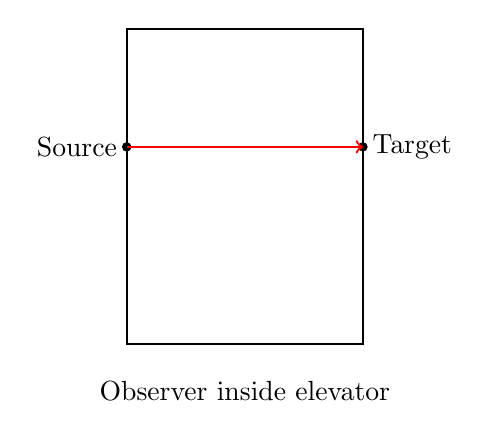
\begin{tikzpicture}
            % Elevator box
            \draw [thick] (0,0) rectangle (3,4);
            % Source and target
            \filldraw [black] (0,2.5) circle (1.5pt) node[left] {Source};
            \filldraw [black] (3,2.5) circle (1.5pt) node[right] {Target};
            % Light beam (straight)
            \draw [red, thick, ->] (0,2.5) -- (3,2.5);
            % Subtext
            \node at (1.5, -0.6) {Observer inside elevator};
        \end{tikzpicture}
        \caption{Freefall (Elevator's Frame)}
    \end{subfigure}
    \hfill
    % --- Subfigure 2: Freefall (Ground Frame) ---
    \begin{subfigure}[b]{0.45\textwidth}
        \centering
        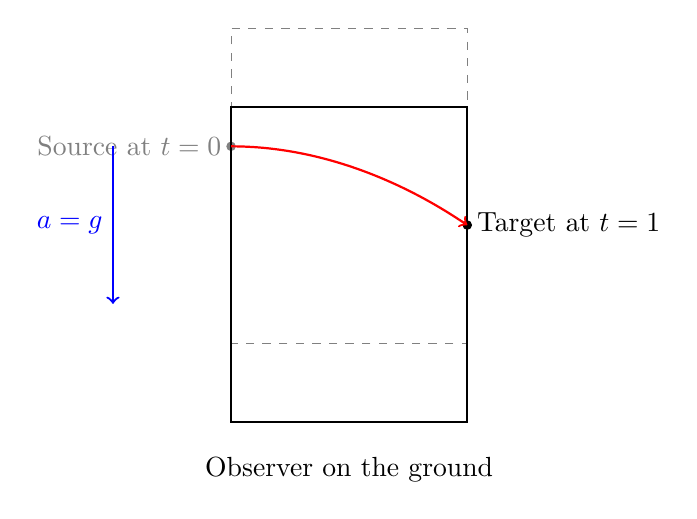
\begin{tikzpicture}
            % Initial Elevator (dashed)
            \draw [dashed, gray] (0,1) rectangle (3,5);
            \filldraw [gray] (0,3.5) circle (1.5pt) node[left] {Source at $t=0$};

            % Final Elevator (solid)
            \draw [thick] (0,0) rectangle (3,4);
            \filldraw [black] (3,2.5) circle (1.5pt) node[right] {Target at $t=1$};

            % Motion arrow
            \draw [->, thick, blue] (-1.5, 3.5) -- (-1.5, 1.5) node[midway, left] {$a = g$};

            % Light beam (parabola curving downwards)
            \draw [red, thick, ->] (0,3.5) parabola (3,2.5);

            % Subtext
            \node at (1.5, -0.6) {Observer on the ground};
        \end{tikzpicture}
        \caption{Freefall (Ground Frame)}
    \end{subfigure}

    \vspace{1cm}

    % --- Subfigure 3: Stationary in Space ---
    \begin{subfigure}[b]{0.45\textwidth}
        \centering
        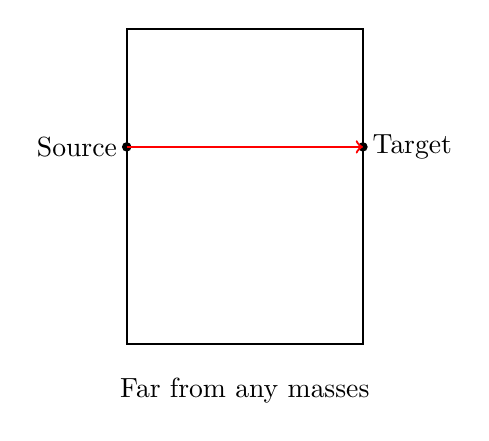
\begin{tikzpicture}
            % Elevator box
            \draw [thick] (0,0) rectangle (3,4);
            % Source and target
            \filldraw [black] (0,2.5) circle (1.5pt) node[left] {Source};
            \filldraw [black] (3,2.5) circle (1.5pt) node[right] {Target};
            % Light beam (straight)
            \draw [red, thick, ->] (0,2.5) -- (3,2.5);
            % Subtext
            \node at (1.5, -0.6) {Far from any masses};
        \end{tikzpicture}
        \caption{Stationary in Deep Space}
    \end{subfigure}
    \hfill
    % --- Subfigure 4: Stationary on Earth ---
    \begin{subfigure}[b]{0.45\textwidth}
        \centering
        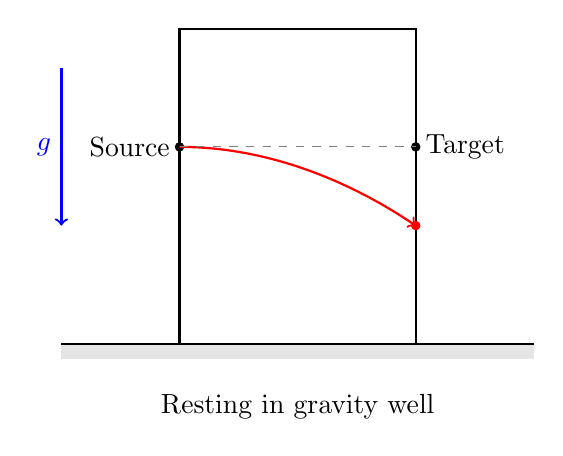
\begin{tikzpicture}
            % Ground / Earth surface
            \fill [gray!20] (-1.5, -0.2) rectangle (4.5, 0);
            \draw [thick] (-1.5, 0) -- (4.5, 0);

            % Elevator box
            \draw [thick] (0,0) rectangle (3,4);

            % Gravity arrow
            \draw [->, thick, blue] (-1.5, 3.5) -- (-1.5, 1.5) node[midway, left] {$g$};

            % Source and intended target
            \filldraw [black] (0,2.5) circle (1.5pt) node[left] {Source};
            \filldraw [black] (3,2.5) circle (1.5pt) node[right] {Target};

            % Light beam (bends down due to gravity)
            \draw [red, thick, ->] (0,2.5) parabola (3,1.5);

            % Dashed line showing straight path
            \draw [dashed, gray] (0,2.5) -- (3,2.5);
            % Actual hit point
            \filldraw [red] (3,1.5) circle (1.5pt);

            % Subtext
            \node at (1.5, -0.8) {Resting in gravity well};
        \end{tikzpicture}
        \caption{Stationary on Earth}
    \end{subfigure}

    \caption{Einstein's equivalence principle: The effects of being in a stationary gravitational field (d) are locally indistinguishable from an accelerating frame, whereas freefall in a gravitational field (a/b) creates a locally inertial frame similar to deep space (c).}
    \label{fig:einstein_elevator}
\end{figure}